\chapter{基于多粒度切分的局部对齐网络}

\section{引言}
近年来,局部信息在计算机视觉的各种任务中发挥着越来越重要的作用,除了服装图像检索之外,这些任务还包括但不限于:细粒度分类、行人重识别、
视觉问答等。细粒度分类用于在一个大的类别中区分不同的小的类别,比如识别具体的鸟的品种,这需要着重对鸟的一些关键部位(比如嘴巴、眼睛)
做特征学习\cite{wang2018learning};类似的,行人重识别需要抽取行人特定部位(如头部、肩膀、腿部)的信息以消除因姿势不同带来的全局信息的偏差\cite{sun2018beyond};视觉问答任务里,
输入为一幅图像和与这幅图像相关的任何一个问题,算法需要输出这个问题的答案,需要对这幅图有全局的语义理解,同时根据问题侧重的学习相关的局部信息特征。
视觉问答的输入图像一般包括多个实例,输入问题有可能只关注其中的一部分,因此对局部信息的提取可以用目标检测框出所有的实例\cite{anderson2018bottom},而细粒度分类以及
图像检索任务一般涉及单个实例,需要采取不同的策略。

对单个实例的局部信息的学习一般有两种方式:基于软注意力(Soft attention)以及基于硬注意力(Hard attention)。软注意力指对图像不同区域的特征赋予不同大小的权重
,本文第三章提出的网络设计方式就是一种基于软注意力机制的方法,通过学习注意力权重分布图自适应的根据输入调节局部特征的权重以达到对局部信息的抓取,这种方法一般不需要
额外的标注信息去监督;硬注意力本质为软注意力机制的特征形式,软注意力的权重值是连续的(一般为0到1之间),而硬注意力机制则是0——1分布,即只保留部分局部区域的信息,
舍弃其余的信息。基于硬注意力机制的做法一般是通过对原图的切分来实现的,Wei等人提出一种基于关键点的切分方法\cite{wei2017glad},根据关键点所定位出的部件位置
生成检测框,随后再根据检测框对原图裁剪输入网络提取这部分的局部信息,这种方式有一定的有效性,但是需要依赖关键点的标注,对资源消耗较大。Li等提出一种无需额外标注
(只需要类别信息的标签)的切分方式\cite{li2017learning},其做法是直接对输入的图像横向平均切分,将每一个图像切片以及完整的原图送入网络做分类学习,且使用了不同大小的
卷积核对输入进行多尺度信息提取。

本章介绍一种具有创新性的基于切分的局部对齐网络结构,传统的基于切分去学习局部特征的做法大多数是对原图做切分,这种切分方式旨在通过对保留下的局部信息单独训练以达到增强
其语义强度的目的,但是这种直接舍弃大部分图像信息的方式不利于网络收敛,甚至会导致模型的过拟合,基于此弊端提出一种对特征图的切分方式。在此基础上对切分策略做了多方面的
改进,在强化局部特征语义信息的同时做到局部区域更好的对齐。
\section{方法与实现}
所提出的网络框架如图\ref{fig:MGN}所示,输入图像首先经过特征提取器提取特征,此处的特征提取器指基础网络(如ResNet)去除最后的全局池化层以及之后的部分,
输出的特征是一个张量,随后该特征复制若干份,并进入四个并行的分支:Global、Horizontal、Vertical、Annular。其中Global为全局分支,学习全局语义信息,
其余三个分支为局部分支,学习局部特征。
\begin{figure}[h]
  \centering
  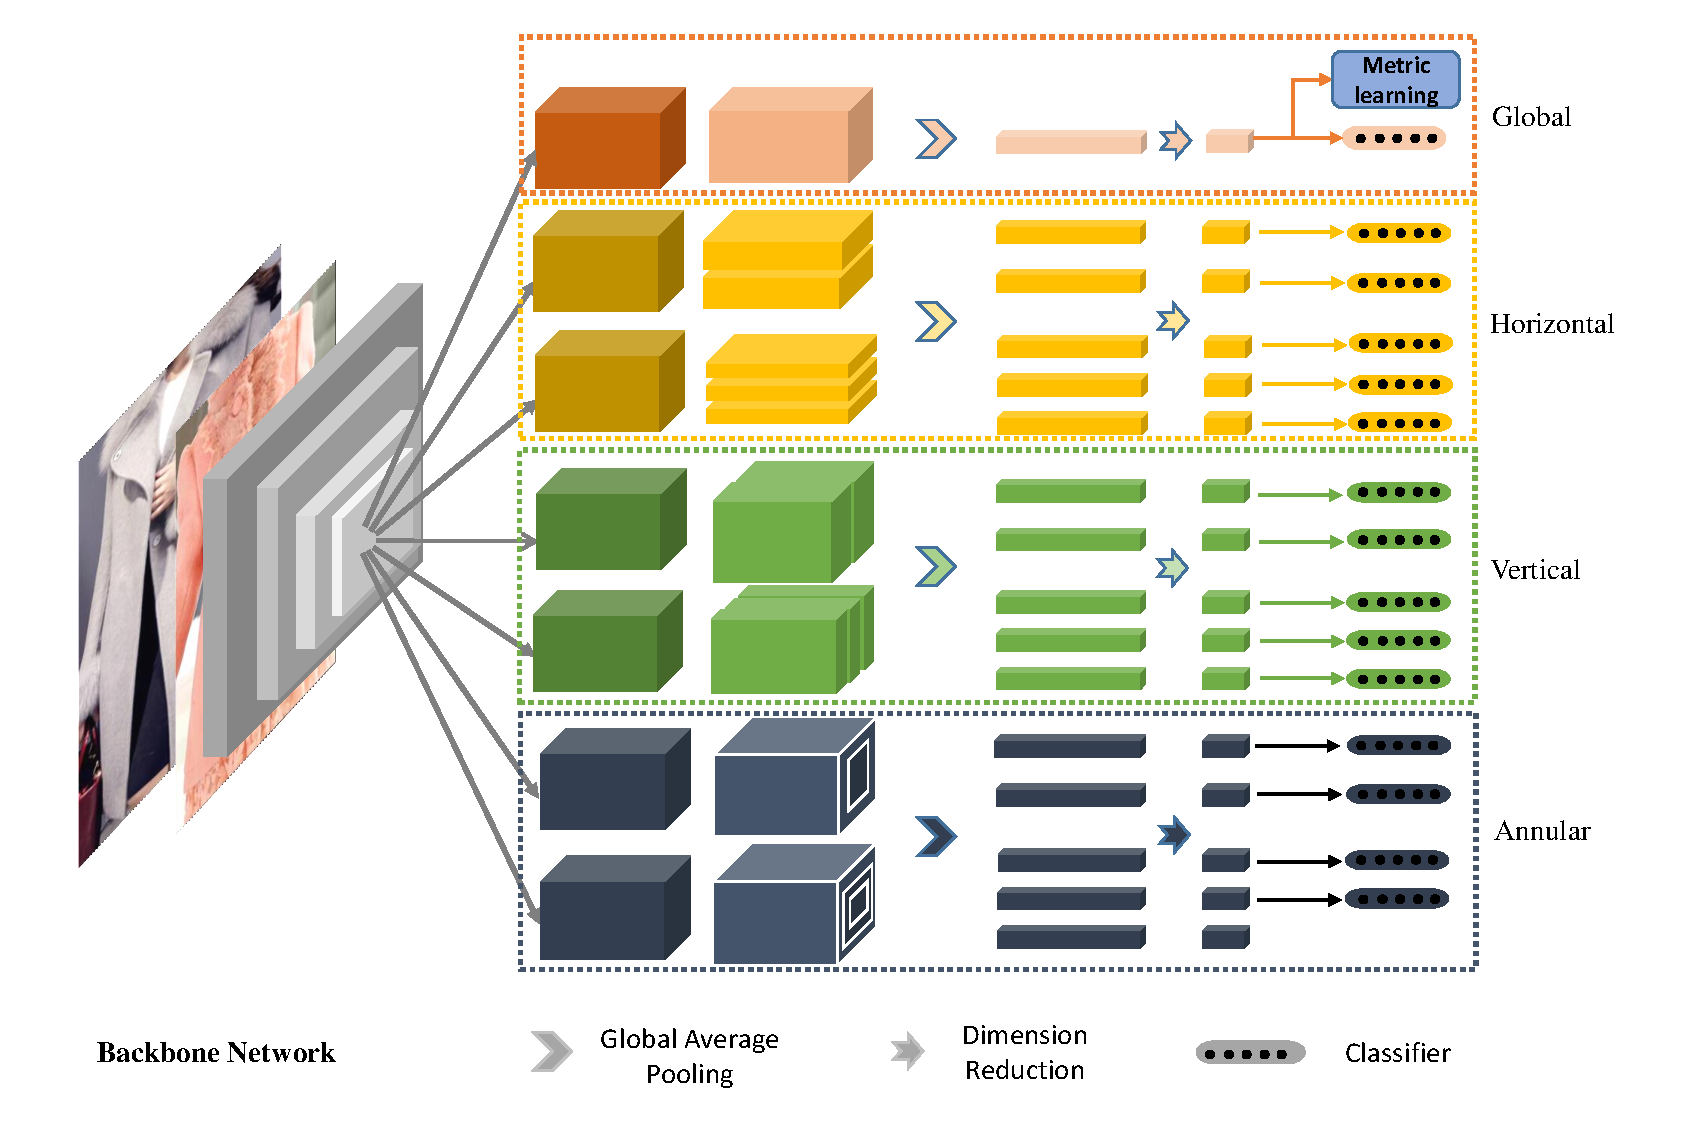
\includegraphics[width=1.0\linewidth]{Img/MGN.pdf}
  \caption{基于切分的局部对齐网络框架图}
  \label{fig:MGN}
\end{figure}

\subsection{对特征图的切分}
传统的基于切分的方式去学习局部特征的做法大多数是对原图做切分,然后将每个图像切片送入网络单独处理,而在本章所提出的方法中,切分操作是对特征图实施,如图\ref{fig:MGN}
中的局部分支所示。我们认为对原图切分之后保留的局部图像切片语义信息不够丰富,直接代表图像去识别其类别可能会导致过拟合,而基于特征图的切分则与之不同,
得益于卷积操作的特性,每个特征切片有着更丰富的上下文信息。
\begin{figure}[h]
  \centering
  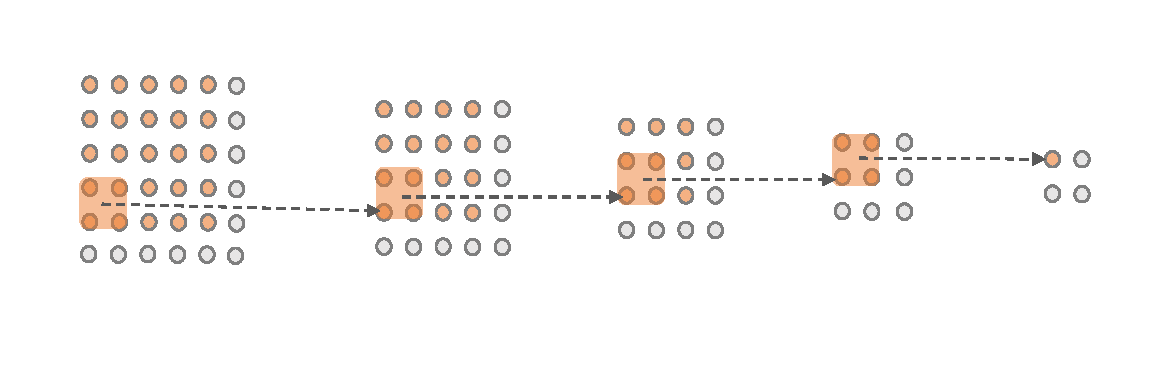
\includegraphics[width=1.0\linewidth]{Img/RF.pdf}
  \caption{卷积操作与感受野}
  \label{fig:RF}
\end{figure}


感受野(Receptive Field)是深度神经网络中的一个很常见的概念,它代表在特征图上的像素点映射到原图后的区域大小。而特征图上某个像素点的感受野的大小并不能按照原图和特征图大小的比例直接计算,
这是由卷积操作的特性所决定的,当前层的感受野与之前所有卷积层的参数都有关系。以图\ref{fig:RF}为例,假设输入图像大小为$6 \times 6$,经过四次卷积层,卷积核大小均为
$2 \times 2$,步长均为$1$,最后得到$2 \times 2$的输出,由图中感受野的变化情况可以看出:最后一层的输出特征图每个像素点对应的感受野对应原图的$5 \times 5$大小区域。

\begin{figure}[h]
  \centering
  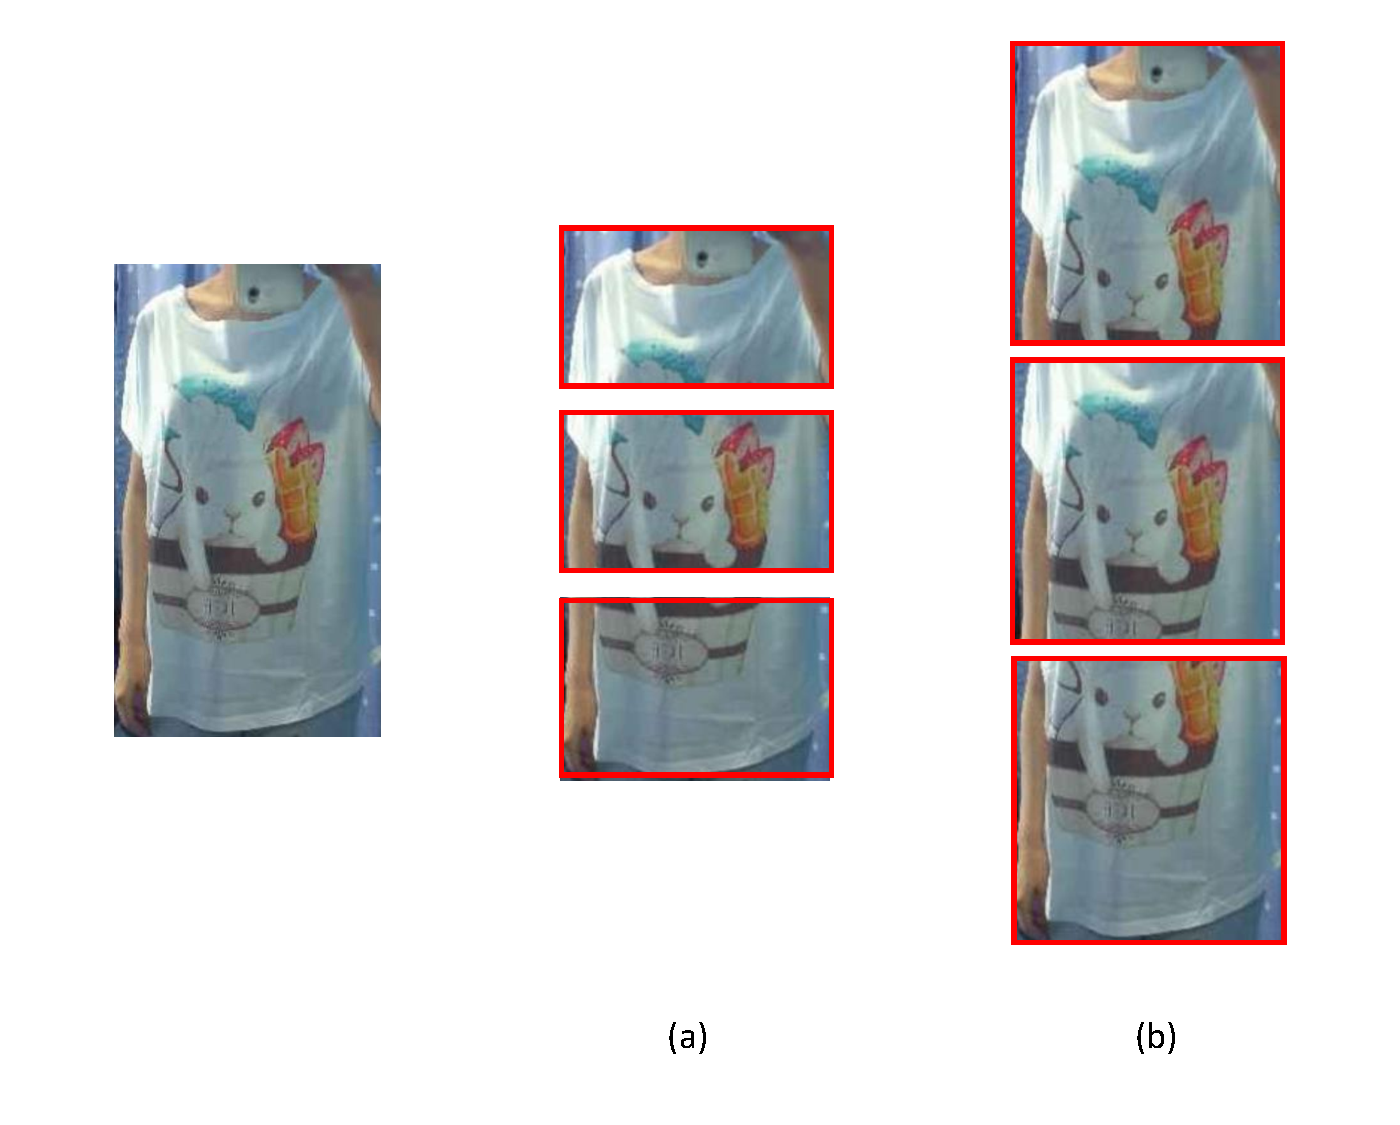
\includegraphics[width=0.8\linewidth]{Img/RFcmp.pdf}
  \caption{对原图切分和对特征切分的理论感受野差别}
  \label{fig:RFcmp}
\end{figure}

上述例子说明对特征图的切分和对原图的切分有根本区别,对特征图切分得到的特征切片包含了原图对应比例区域之外的上下文信息,如图\ref{fig:RFcmp}中,(a)、(b)分别代表
对原图和特征图切分后每个切片对应的理论感受野。然而,以(b)中所示感受野大小为准(有重叠区域)去切分原图和对特征图的切分仍然是不同的,
理论上来说,虽然特征图的每个切片对应的感受野比其在整个特征图所占比例在原图对应区域要大,但是这个区域的信息强度分布并不是平均的。Luo等人指出,卷积神经网络中的理论
感受野与实际感受野有很大差别,实际上来说越是靠近感受野中心的区域信号强度越大,整体呈高斯分布\cite{luo2016understanding}。因此,特征图的特征切片在包含更多的上下文
信息的同时,局部信息可以以相对更强的信号强度表达出来,而直接用有重叠区域的方式对原图切分反而会引入过强的噪音,导致不利于局部信息的表达。

我们对特征提取网络输出的张量进行切分,随后对每个切片进行全局最大池化(Global Max Pooling)得到若干向量,其维度为原特征图的通道数,然后用$1 \times 1$大小的卷积核对这个向量降维,
最后以降维后的向量作为局部特征的表示送入分类器学习原图的类别。分类器对应的损失函数就是Soft Max Loss,这么做的出发点是希望网络可以仅通过输入图像的某个局部区域去区分
其类别,这样可以提高局部区域特征的表达能力。所以,局部分支最后的特征由多个局部切片的向量组成:$\mathcal{F}=\{S_{1},S_{2}\cdots S_{i}\}$,
则该分支的损失为$i$个Soft Max Loss的均值。
\subsection{环形切分}
图\ref{fig:MGN}中,根据对特征切分的实施方式不同,局部分支共有三个:Horizontal(横向切分)、Vertical(纵向切分)、Annular(环形切分)。环形切分是本方法所提出的一种
创新型的切分方式,这三种切分方式的具体实现方式区别如图\ref{fig:annular}所示。图中示例均为三等份的切分,横向或者纵向的切分比较直接,只需在特征图的三等分点进行切割。
环形的切分方式则是按照特征图边缘到特征图中心长度的三等分点,按照“回“字形切分出环形的特征,确切的来说,得到的是外侧的切片为环形、最里侧的切片为矩形的特征。
\begin{figure}[h]
  \centering
  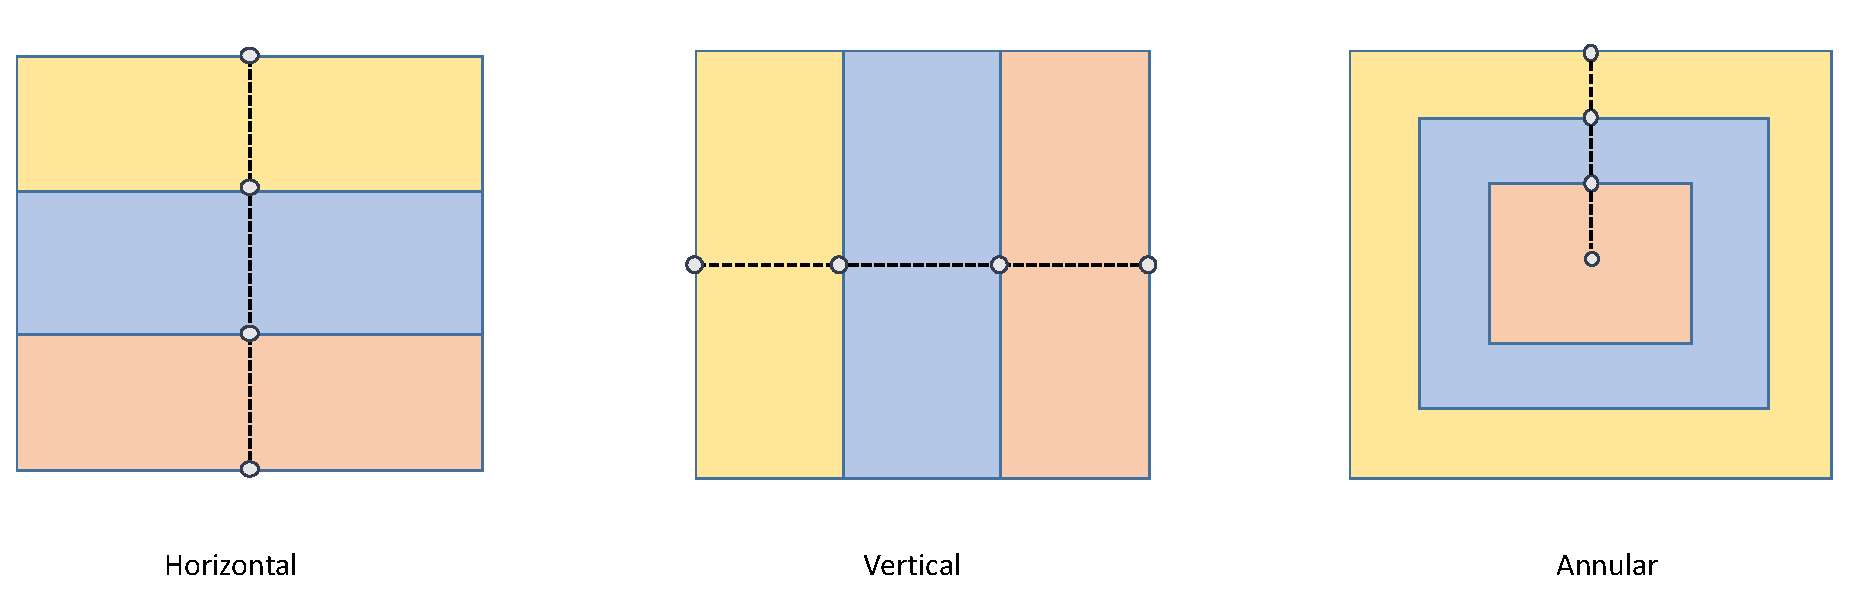
\includegraphics[width=1.0\linewidth]{Img/annular.pdf}
  \caption{对特征图的不同切分方式}
  \label{fig:annular}
\end{figure}


使用环形切分方式的出发点是基于实际场景,服装图像的空间分布多种多样,其中有很多一部分是类似图\ref{fig:annular-vis}中的结构:服装最显著的局部特征位于中心区域,且环形区域内对应有完整的局部区域特性,图中最中心的区域是一个红心的标识,中间的环形有完整的“PLAY”字样,最外的一个环则是衣服领口和袖子的纹理等特性。
这种情况下,横向的切分方式难以保证关键局部信息的完整性,而所提出的环形切分方式可以很好的解决这类问题。此外,环形切分的方式还具有很强的旋转不变性,尤其是对于图像的
中心区域,这种特性可以有效防止图像拍摄的角度偏差所带来的影响,使得模型具有很强的泛化能力。图\ref{fig:annular-vis}中展示了环形切分对旋转因素的有效对抗,原图在旋转
90\degree、180\degree、270\degree 的情况下,环形切分所得到的特征切片的内容不会发生改变,即使在旋转45\degree 的极端情况下,图像的中心区域(也是最显著的局部区域)
的特征切片依然不会有大幅度的改变。
\begin{figure}[h]
  \centering
  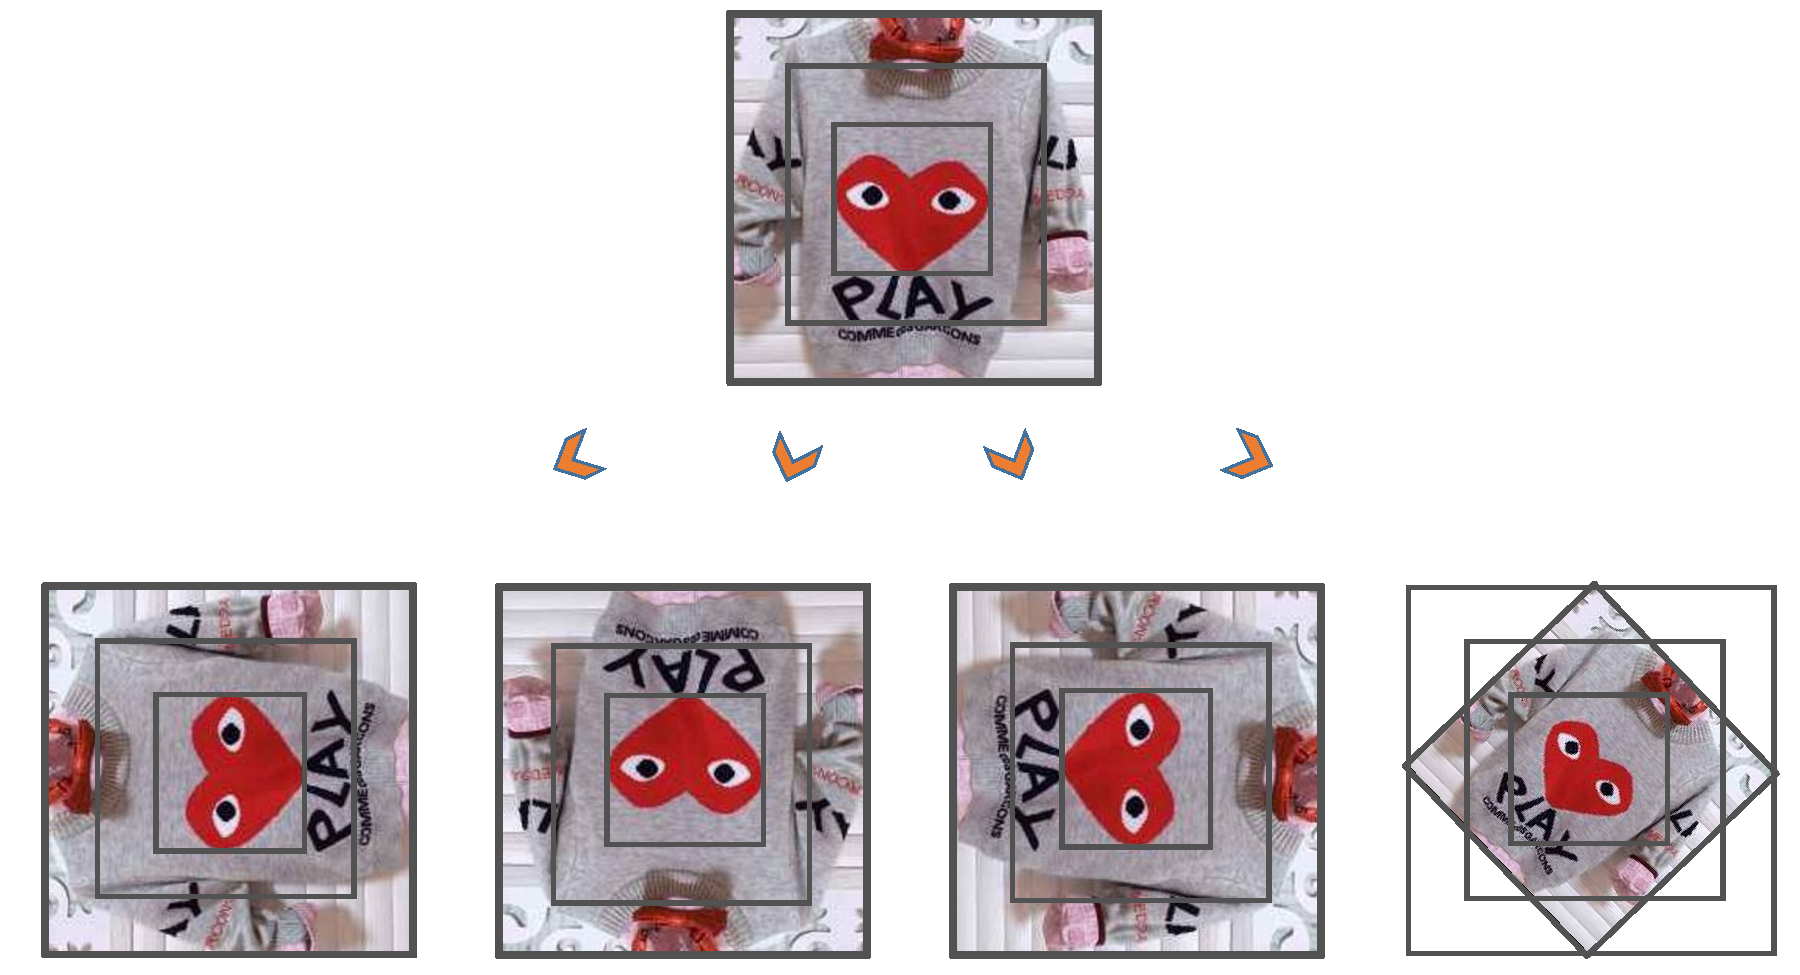
\includegraphics[width=1.0\linewidth]{Img/annular-vis.pdf}
  \caption{环形切分方式的旋转不变性}
  \label{fig:annular-vis}
\end{figure}


此外,横向切分、纵向切分和环形切分的组合方式可以有效提升特征的表达能力。考虑到服装款式的多样性,单一的切分方式不能保证能得到匹配服装图像空间分布的最优特征切片,
而三种切分方式的组合可以对局部特征做更加全面的提取,大大提高了最优特征切片的表达能力,有利于局部区域的对齐。
\subsection{多粒度切分}
本小节介绍一种对特征图使用不同粒度(即多粒度)的切分策略,可以有效提升最终特征的语义表达能力,此处粒度可以理解为尺度或者密度。

\begin{figure}[h]
  \centering
  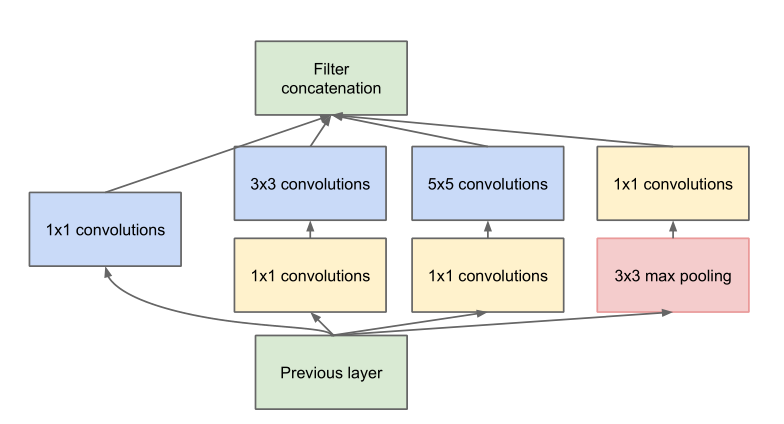
\includegraphics[width=0.75\linewidth]{Img/Inception.png}
  \caption{Inception模块的多尺度卷积}
  \label{fig:Inception}
\end{figure}

本方法受启发于GoogLeNet,图\ref{fig:Inception}描述了GoogLeNet的核心模块的设计方式,对于输入的特征图采用$1 \times 1$、$3 \times 3$、$5 \times 5$三种尺度的卷积核以及一个最大池化层的多路并行分支
提取特征,虽然通过不同的Padding方式可以得到相同大小的特征图输出,但是输出特征的每个像素点对应的感受野却不相同。最后对多个分支的特征图输出在通道维度拼接起来,获得
语义信息更丰富、表达能力更强的特征输出。

类似的网络设计理念还被应用在目标检测和语义分割等领域。目标检测任务中,特征金字塔网络(Feature Pyramid Network, FPN)取得了很大的成功\cite{lin2017feature},其网络设计包含自底向上和自顶向下两个路径
,自底向上即常见的卷积神经网络提取高层语义信息,而自顶向下的过程则是通过上采样逐层放大特征图的分辨率,并且通过阶跃连接和自底向上的特征图融合以修正细节信息,如图\ref{fig:fpn}。最后RPN
层的Anchor取自不同分辨率的特征图。分辨低的层语义信息丰富,有利于大目标的检测;分辨率高的层细节信息丰富,有利于小目标的检测。
\begin{figure}[h]
  \centering
  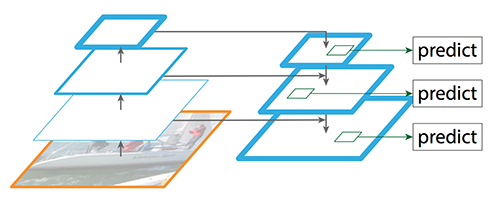
\includegraphics[width=0.75\linewidth]{Img/fpn.png}
  \caption{特征金字塔网络\cite{lin2017feature}}
  \label{fig:fpn}
\end{figure}


所提出的多粒度切分方法对特征图按照不同的密度(尺度)切分,不同的切分粒度可以得到不同大小的特征切片,他们所包含的语义信息也有所区别,这些特征切片分别输入分类器进行
分类训练。在测试阶段,这些感受野不同的局部特征切片拼接为一个整体(池化以后的向量),融合了不同尺度的局部特征信息,获得更强的表达能力。图\ref{fig:sg-mg}以横向切分
为例对比了单粒度切分与多粒度切分在实施时的区别,图中每个虚线框框出的部分代表一种切分粒度,且每个虚线框的输出都是由相同的特征图复制得到
,不同的切分粒度对应不同数量的特征切片数目。理论上来说,不同切分粒度的数量没有限制,但是不同的切分粒度带来更多的特征切片,这也会导致最终拼接的特征维度变得很高
,所以需要在模型性能和特征维度之间作出权衡。
\begin{figure}[h]
  \centering
  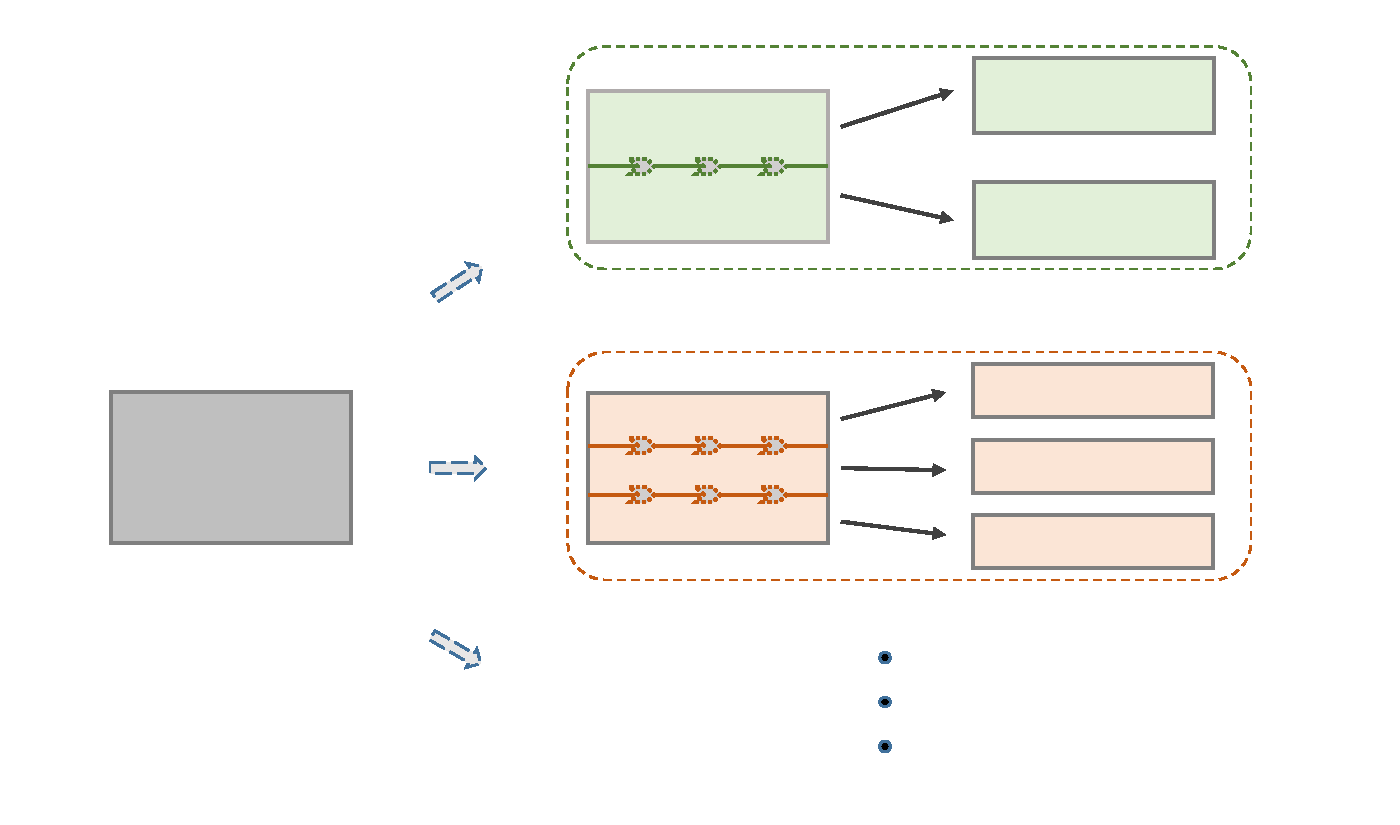
\includegraphics[width=1\linewidth]{Img/sg-mg.pdf}
  \caption{单粒度切分与多粒度切分的对比图}
  \label{fig:sg-mg}
\end{figure}

\section{实验与分析}
\subsection{实验设定}
